% SPDX-License-Identifier: Apache-2.0
% Generated by publication/build_science_figures.py; no experiments are run.
% Frozen inputs: results/confirmation_v2/{confirmation,performance,published_comparator}.json
% Post-confirmation inputs: alternatives/ordering/ordering_results.json
% Alternative inputs: alternatives/matrix_action/matrix_probe_{results,assessment}.json
% External sources: cite keys miller, exact, lorist, davidson, openaiMatrix.
\subsection{Exact agreement and accepted production}

The corrected confirmation completed \textbf{128 tiny instances}, including
\textbf{504 exhaustive table bijections} and \textbf{270 conditioned-output checks}.
Every tiny-instance count agreed with the independent enumerator. Enumerated feasible
tables were compared with the compiler's entire ranked family, including rank/unrank
inverses. These are finite exhaustive checks on the declared cases; they do not replace
the argument that multiplicity-weighted decoding samples the intended labeled law.

The larger campaign completed \textbf{12 synthetic requests} and delivered
\textbf{1,200 accepted tables}: 100 independently cell-checked outputs per request.
Construction took 0.0073--4.6444 seconds in the recorded executions.
The strongest independently written conventional counter completed 11 of
the 12 cases during confirmation, with matching counts in each. Its last case
timed out. The remaining count was corroborated only in the subsequent ordering
diagnostic described below; it is not retroactively counted as an independent result
of the frozen confirmation.

\begin{figure}[H]
\centering
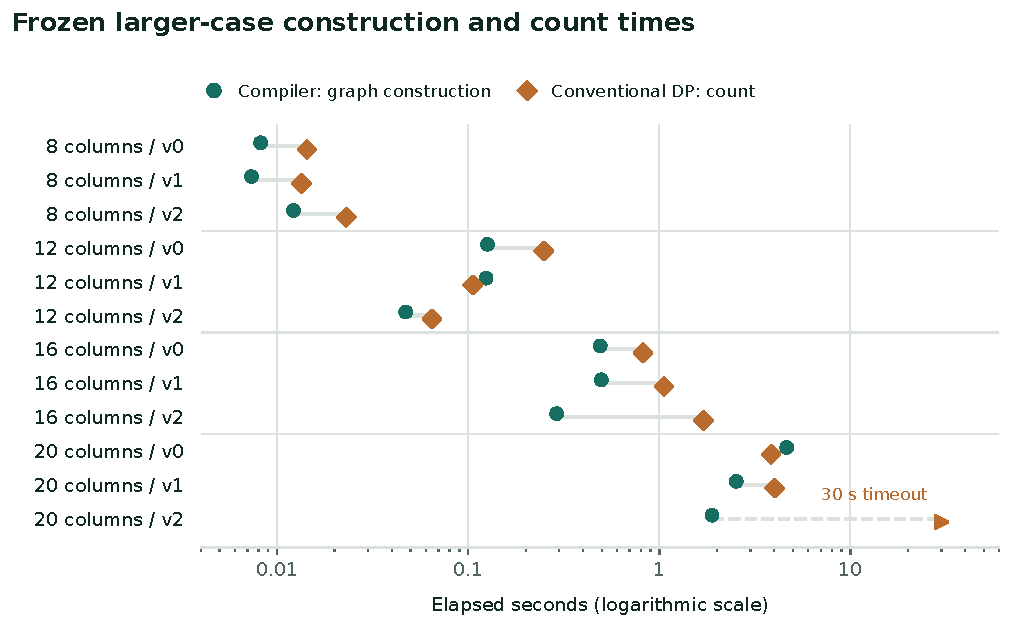
\includegraphics[width=\linewidth]{figures/scientific_performance.pdf}
\caption{All twelve larger cases from the corrected frozen campaign. Variants change
the margins and, for v2, add forbidden cells. Circles measure graph construction;
diamonds measure independent conventional counting. The right-pointing marker is a
30-second timeout, not a completed count. These are single executions, not repeated
performance estimates. Source: the frozen \texttt{performance.json} record.}
\label{fig:scientific-performance}
\end{figure}

\begin{table}[H]
\centering\small
\begin{tabular}{@{}rrrrr@{}}
\toprule
Columns & Exact labeled tables & Graph states & Compiler (s) & Conventional (s)\\
\midrule
8 & $20\,322$ & 106 & 0.0082 & 0.0143\\
12 & $14\,875\,620$ & 367 & 0.1262 & 0.2486\\
16 & $12\,763\,583\,010$ & 1,012 & 0.4913 & 0.8237\\
20 & $11\,973\,051\,233\,892$ & 2,354 & 4.6444 & 3.8548\\
\bottomrule
\end{tabular}
\caption{The four regular v0 controls, with four rows and column totals of two.
Both symmetry-aware implementations return the displayed counts. Large family size
is an output property; it does not by itself demonstrate algorithmic novelty.}
\label{tab:scientific-regular}
\end{table}

The simpler labeled-cell counter completed the three eight-column cases and reached
its state budget on the other nine. This comparison supports the usefulness of
column symmetry on these inputs. The independent orbit counter uses the same known
structural principle and is the more consequential conventional comparison.

\subsection{A published counterexample and a charged ordering repair}

The published $13\times17$ Darwin-finch binary-margin problem provides an external
check on the scope of the implementation. The authors' actual EXACT source, with
documented Python-3 compatibility edits, returned
\(67\,149\,106\,137\,567\,626\) in \textbf{0.40397 seconds}.
The new bounded compiler refused at its declared state/transition budget after
20.32 seconds. This is a successful conventional computation on a task
the constructed implementation did not complete. The published software's binary
scope is respected; unsupported arbitrary-cap tasks are not scored as incorrect
outputs~\cite{miller,exact}.

The final larger confirmation case initially appeared more favorable: the compiler
completed construction in 1.890 seconds while the conventional reference
timed out at 30 seconds. A separate post-confirmation challenge copied that reference
and changed only its row-order parameter. All 24 row permutations received the same
3.5-second execution budget. Eight finished, all returning
\(37\,877\,767\,916\); sixteen timed out. The best order took
\textbf{1.724 seconds}, and the ascending-row-sum permutation took 1.814 seconds.
Thus an ordinary ordering change reaches the compiler's recorded construction scale
on this observed case, without a new recurrence or pruning rule.

The entire diagnostic cost \textbf{75.177 seconds}, including unsuccessful
attempts. That search cost cannot be replaced by the winning attempt's runtime in a
first-use comparison. No general ordering policy was selected, and this adaptation
is not a fresh held-out result. The comparator returns a count; the compiler also
constructs a reusable transition graph. The small timing differences therefore do
not establish robust superiority in either direction.

\subsection{A second production route, executed and rejected}

The investigation also constructed an actual polynomial-action operator for
\(e^A v\), motivated by the sharp complete Crouzeix bound reported in OpenAI
family 325~\cite{openaiMatrix}. It executed 144 matrix/tolerance cases over
48 matrices: Jordan, symmetric diffusion, and two nonnormal convection-diffusion
families, at dimensions 16--128 and absolute tolerances $10^{-6}$, $10^{-10}$,
and $10^{-12}$. All produced vectors met their thresholds against a numerical
\texttt{expm} reference. Representative inputs, outputs, and reference vectors are
preserved, so this was a production probe rather than a certificate-only proposal.

The proposed theorem dependency fails a stronger prior-art check. The scalar
Crouzeix constant two needed by \(e^A v\) was already public in August 2026;
the newly complete matrix-valued scope is unused here~\cite{lorist}.
More decisively, this implementation encloses the numerical range in a disk.
The classical numerical-radius dilation and Okubo--Ando result already make that
disk a \emph{complete} 2-spectral set. Consequently the entire constant-two
polynomial program is also an existing conventional construction, with the same
degree, recurrence, and output~\cite{davidson}.

\begin{figure}[H]
\centering
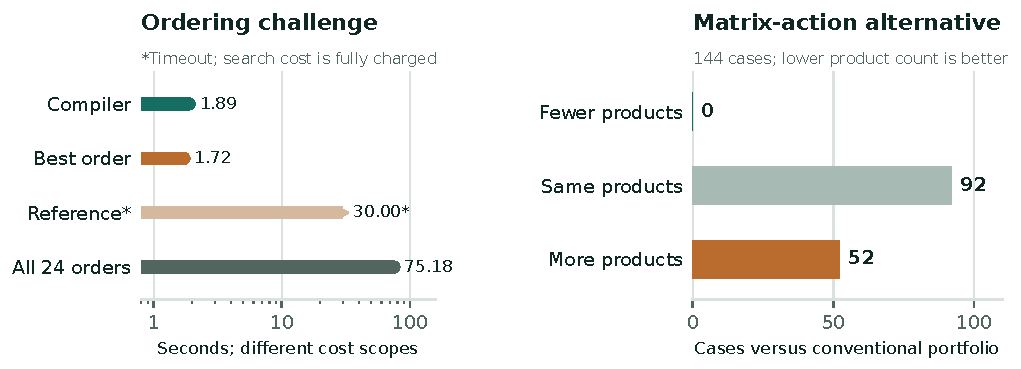
\includegraphics[width=\linewidth]{figures/scientific_challenges.pdf}
\caption{Two challenges after the frozen confirmation. Left: the ordering diagnostic
separates the winning conventional execution from the charged 24-order search;
the 30-second reference point is the original censored confirmation result.
Right: the executable matrix-action candidate uses fewer, equal, or more products
than a conventional portfolio containing the identical classical disk bound,
operator-norm bounds, normal-matrix bounds, and Jordan nilpotency. The portfolio
comparison is by degree, not a measured optimal portfolio runtime.}
\label{fig:scientific-challenges}
\end{figure}

Against the weaker general multiplier $1+\sqrt2$, substituting two saved one
matrix-vector product in 18 cases: 4,194 products became 4,176,
an aggregate reduction of 0.43\%. Against the stronger conventional
portfolio, the candidate had \textbf{0 lower-degree cases, 92 ties, and 52 higher-degree
cases}. These results do not qualify a new productive operator. The recorded error
bound controls analytical truncation only; ordinary floating-point evaluation and
a numerical reference do not provide total roundoff certification. This route was
therefore rejected as the next flagship rather than promoted on its tighter bound.

{\small\color{muted}Evidence files: the frozen confirmation directory; the
byte-preserved dossiers in \path{alternatives/ordering/} and
\path{alternatives/matrix_action/}. Figure generation reads those records and runs
no new scientific experiment.}
